\chapter{اجزای مورد استفاده در سیستم ردیابی}
%\thispagestyle{empty}

\section{مقدمه}
هدف اصلی پروژه ما طراحی و پياده‌سازی سامانه‌ای است كه بتوان توسط آن موقعيت دقيق و مسير حركت هر جسم متحرك را در هر زمان تعيين كرد. سامانه ذکر شده باید علاوه بر عملکرد مناسب، از لحاظ هزینه هم به صرفه باشد.


برای این که بتوانیم چنین سامانه‌ای را طراحی کنیم اول باید نیازمندی‌های سامانه را تشخیص دهیم، معماری کلی سامانه موردنظر خود را به دست آوریم و سپس با استفاده از این معماری و نیازسنجی انجام شده برای پیاده‌سازی از ماژول‌های مناسب استفاده کنیم. در این فصل در قسمت ۳-۲ ابتدا طرح کلی سامانه ردیابی را توضیح می‌دهیم و سپس در بخش ۳-۳ اجزاء مورد استفاده در این طرح را معرفی می‌کنیم.
\section{طراحی و معماری سیستم}
در این قسمت به طراحی سیستم خود می‌پردازیم. با توجه به نیازمندی‌های پروژه باید ماژول‌های فرستنده و گیرنده، پروتکل ارتباطی و برنامه کاربردی برای نمایش اطلاعات را مشخص کنیم.
هدف اصلی یک سیستم ردیابی این است یک شی خاص را ردیابی کرده و مسیر حرکت آن را در هر زمانی بدست آوریم. در واقع سیستم ردیابی اطلاعاتی درباره مکان فعلی و سرعت شی مورد نظر را در اختیار ما می‌گذارد. در انجام انی پروژه ارتباط ما به صورت یک‌طرفه بوده است، به این صورت که به طور پیوسته مختصات مکانی شی متحرک اندازه گرفته می‌شود و به یک سرور فرستاده می‌شود و سپس پردازش‌های لازم در سمت سرور بر روی این اطلاعات صورت می‌گیرد. با توجه به توضیحات گفته شده می‌توان به سه قسمت اصلی در این سیستم اشاره کنیم \cite{bidabad}:
\begin{itemize}
	\item
بدست آوردن موقعیت مکانی شی متحرک با استفاده از ماژول جی پی اس
	\item
	ارسال اطلاعات مکانی به سرورهای نرم‌افزاری توسط مودم جی اس ام
	\item
	ذخیره اطلاعات مکانی در سمت سرور و پیاده‌سازی برنامه کاربردی برای نمایش مسیر حرکت شی بر روی نقشه
\end{itemize} 
همانطور که دیدیم معماری سیستم ما دارای چهار بخش اصلی است. بخش اول مربوط به گرفتن موقعیت مکانی شی از ماهواره با استتفاده از ماژول جی پی اس است. بخش دوم مربوط به ارسال اطلاعات دریافتی به سرور با استفاده از مودم جی اسم ام است و بخش سوم هم توسعه برنامه کاربردی است که با استفاده از اطلاعات دریافت شده موقعیت شی مورد نظر نمایش داده می‌شود.

\begin{figure}[!h]
	\centerline{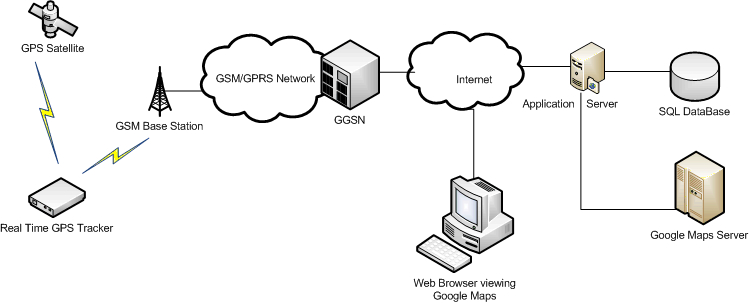
\includegraphics[width=.7\textwidth]{GPS_Tracker}}
	\caption{بلاک دیاگرام سیستم ردیابی \cite{Mohamad2016}}
\end{figure}
شکل ۳-۱ نمای کلی از معماری سیستم طراحی شده و ارتباط بین بخش‌های آن را نشان می‌دهد. برای انتخاب ماژول‌ها لازم است وظیفه هر بخش را دقیق بدانیم و ماژول مورد نظر برای آن را انتخاب کنیم.
\begin{itemize}
	\item 
	در بخش اول لازم است ما موقعیت مکانی شی مورد نظر را به طور پیوسته اندازه بگیریم. در واقع به محض حرکت کردن شی، ماژول جی پی اس به طور پیوسته اطلاعات مکانی و زمانی شی مورد نظر را از ماهواره دریافت می‌کند. سیگنال دریافتی از ماهواره ضعیف می‌باشد و لذا باید از یک آنتن برای تقویت سیگنال مورد نظر استقاده کنیم و در انتها سیگنال تقویت شده که حاوی اطلاعات مکانی و زمانی شی متحرک می‌باشد را به برد آردوینو می‌فرستد.
	\item 
	در بخش دوم اطلاعات ارسالی توسط جی پی اس توسط مودم جی اس ام به سمت سرور فرستاده می‌شود.
	\item 
	سرورهای نرم‌افزاری پس از دریافت اطلاعات آن‌ها را تحلیل می‌کنند. ارتباط ما در این پروژه به صورت یک‌طرفه می‌باشد و درخواستی از سمت سرورهای نرم‌افزاری نخواهیم داشت. در این قسمت پروژه یک نرم‌افزار تحت وب توسعه داده خواهد شد تا بتواند اطلاعات ارسالی را پردازش و ذخیره کند. در قسمت آخر هم این اطلاعات ذخیره شده در صفحه وب طراحی شده نمایش داده می‌شود. 	 
\end{itemize}
\begin{figure}[!h]
	\centerline{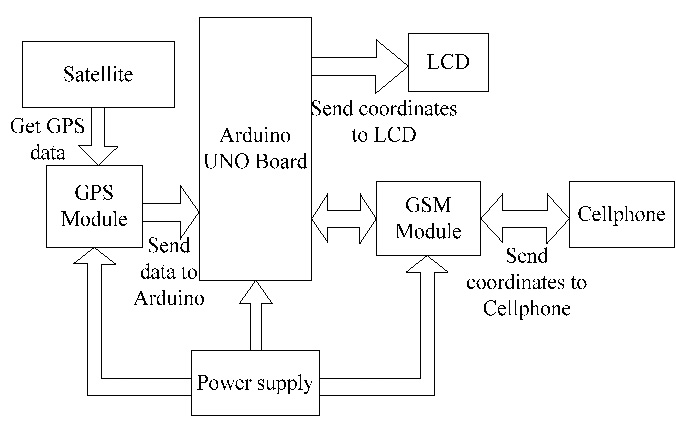
\includegraphics[width=.6\textwidth]{blockdiagram}}
	\caption{معماری سیستم ردیابی پیشنهادی \cite{Rahman2016}}
\end{figure}
\section{اجزاء سیستم}
در قسمت قبل معماري سيستم را مشخص كرديم. حال اجزاء اين معماري را به طور دقيق بيان و معرفي می‌کنیم.
\subsection{اجزاء سخت‌افزاری}
اجزای سخت‌افزاری که برای پیاده‌سازی این سامانه استفاده شده است عبارتند از:
\begin{itemize}
	\item
	ماژول آردوینو
	\item
ماژول سیم ۸۰۸
\RTLfootnote{\lr{SIM 808}}
	\item
	آنتن جی‌پی‌اس
	\RTLfootnote{\lr{GPS Antenna}}
	\item
	آنتن جی‌اس‌ام
	\RTLfootnote{\lr{GSM Antenna}}
\end{itemize}
\subsubsection{ماژول آردوینو}
آردوينو يک ريزپردازنده متن‌‌باز است كه براي نوشتن برنامه‌هايي كه با محیط و اشیا بیرون در تعامل هستند مناسب است. این برد مناسب نمونه‌سازی می‌باشد و نرم افزار و طرح سخت‌افزار آن به صورت آزاد در اختیار تمام افراد قرار گرفته است و هر فرد علاقه‌مند حتی با دانش و تجربه اندک در حوزه الکترونیک مي‌تواند از آردوینو برای انجام پروژه‌های خود استفاده نماید.


آردوينو محیط ساده‌ای براي برنامه‌نويسي دارد كه هر شخصي با اندكي آشنایی با زبان سی\RTLfootnote{\lr{C}} و سی‌ پلاس‌پلاس\RTLfootnote{\lr{C++}} مي‌تواند در این محیط برنامه‌نويسي كند و برنامه نوشته شده را در آردوینو اجرا نماید. به ميكروكنترلر آردوينو ميتوان حسگرهاي مختلف متصل و آن‌ها را كنترل كرد. ریزپردازنده به‌ کار رفته بر روی برد آردوینو بر اساس زبان برنامه‌نویسی آردوینو برنامه‌ریزی شده است و برای کدنویسی به نرم‌افزار یا کامپایلر جانبی نیازی ندارد. 


آردوينو انواع مختلفي دارد كه ما از آردوینو اونو\RTLfootnote{\lr{Arduino Uno R3}} در این پروژه استفاده کرده‌ایم. \lr{R3} سومین و آخرین نسخه آردوینو اونو می‌باشد. برد آردوینو اونو یک میکروکنترلر بر پایه \lr{ATmega328} می‌باشد. ولتاژ كاري آن ۵ ولت مي‌باشد. ولتاژ ورودي این برد می‌تواند در بازه ۷ تا ۲۰ ولت باشد. این برد داراي ۶ پین ورودی آنالوگ، ۱۴ پين ورودي و خروجی ديجيتال، یک پورت یواس‌بی  \RTLfootnote{\lr{USB Port}}، یک ورودی منبع تغذیه و یک دکمه بازنشانی \RTLfootnote{\lr{Reset}} است که اجازه اتصال بردهای توسعه مختلفی را فراهم می‌آورد. \\
در شكل ۳-۱ برد آردوينو \lr{Uno} را مشاهده مي‌كنيد.
\begin{figure}[!h]
	\centerline{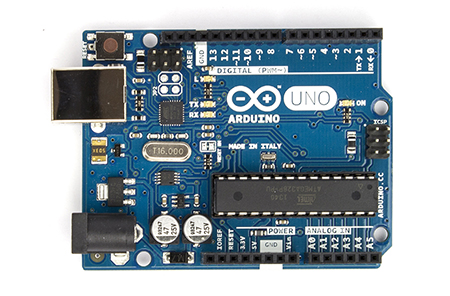
\includegraphics[width=.6\textwidth]{ArduinoUno_R3}}
	\caption{برد آردوینو \lr{UNO R3}}
\end{figure}
\subsubsection{ماژول سیم ۸۰۸}

ماژول سیم ۸۰۸ یک ماژول ترکیبی از جی‌اس‌ام/ جی‌پی‌آر‌اس\RTLfootnote{\lr{GSM/GPRS}} و ماژول  جی‌پی‌اس  با قابلیت پشتیبانی از چهار باند فرکانسی ۸۵۰/۹۰۰/۱۸۰۰/۱۹۰۰ مگاهرتز برای ارسال داده، پیام کوتاه و برقراری تماس صوتی می‌باشد. این ماژول دارای یک سوکت سیم‌کارت می‌باشد که سیم‌کارت در داخل آن قرار می‌گیرد.این ماژول آخرین و جدیدترین محصول شرکت \lr{SIMCOM} می‌باشد که از شبکه چهار باند جی‌اس‌ام/ جی‌پی‌آر‌اس پشتیبانی و برای ردیابی ماهواره‌ای از فناوری جی‌پی‌اس استفاده می‌کند. در واقع با استفاده از مودم جی‌اس‌ام/ جی‌پی‌آر‌اس و ماژول سیم ۸۰۸ می‌توان به تبادل داده روی شبکه جی‌اس‌ام از طریق واسط یو‌اس‌بی پرداخت و از طریق به اطلاعات دستگاه‌های مستقر در مکان‌های دور دسترسی یافت.

طراحی فشرده این تراشه که دو سیستم مخابراتی و موقعیت‌یاب را در یک بسته ادغام می‌کند موجب کاهش هزینه و زمان برای انجام پروژه‌های مبتنی بر جی‌پی‌اس شده است. این ماژول با تکنولوژی ذخیره انرژی \RTLfootnote{\lr{Power Saving}} طراحی شده است و مصرف انرژی آن در حالت خواب بسیار کم در حدود یک میلی آمپر می‌باشد.
 
 
 این ماژول دارای ۶۸ پین، سوکت یو اس بی، سیم‌کارت، بلوتوث می‌باشد. دارای حساسیت بالای دریافت موقعیت جهانی با ۲۲ کانال ردیابی و ۶۶ کانال گیرنده می‌باشد. علاوه بر این از \lr{A-GPS} پشتیبانی می‌کند که برای موقعیت‌یابی داخل ساختمان استفاده می‌شود. این ماژول توسط فرمان \lr{AT} کنترل می‌شود و از سطح منطقی ۳.۳ تا ۵ ولت پشتیبانی می‌کند \cite{datasheet}.\\ از جمله ویژگی‌های این تراشه می‌توان موارد زیر را نام برد:
\begin{itemize}
	\item 
	پشتیبانی از سیم‌کارت تمامی آپراتورها
	\item
	دارای مدار کنترل شارژ
	\item
	پشتیبانی از فرکانس ساعت
	\item 
	پشتیبانی از کانال‌های آنالوگ
	\item
	کم‌مصرف (۱ میلی آمپر در حالت خواب)
	\item 
	ولتاژ ورودی ۳.۴ تا ۴.۴ ولت
	\item 
	قابلیت نصب ۳ آنتن جی‌پی‌اس، جی‌اس‌ام و بلوتوث
\end{itemize}
در شکل ۳-۲ و ۳-۳ این تراشه را مشاهده می‌کنید.
\begin{figure}[!h]
	\centerline{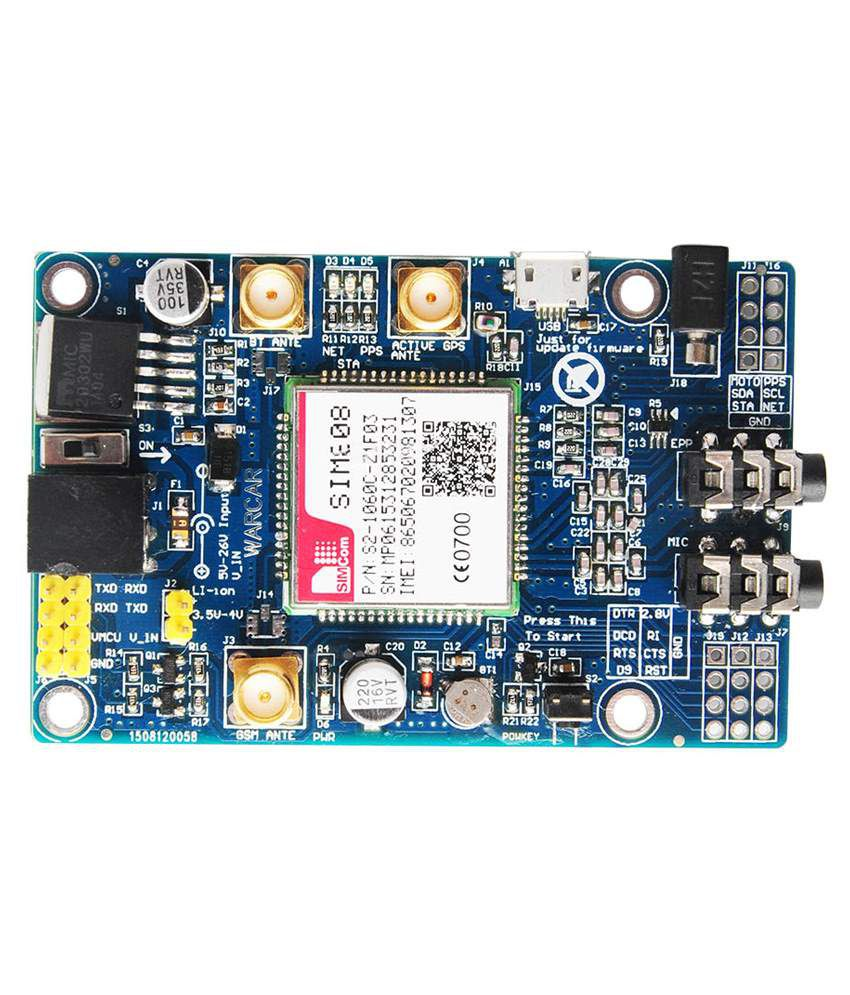
\includegraphics[width=.6\textwidth]{sim808}}
	\caption{نمایی از قسمت روبرو تراشه \lr{SIM 808}}
\end{figure}
\\
\begin{figure}[!h]
	\centerline{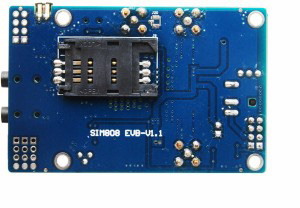
\includegraphics[width=.6\textwidth]{backside-sim808}}
	\caption{نمایی از قسمت پشت تراشه \lr{SIM 808}}
\end{figure}

\subsubsection{آنتن \lr{GPS}}
بهتر است قبل از معرفي آنتن \lr{GPS}، شيوه موقعيت‌يابي توسط سيستم موقعیت‌یاب جهانی \RTLfootnote{\lr{GPS}} را به طور مختصر توضيح بدهيم. سيستم \lr{GPS} در واقع شامل ۲۷ ماهواره است كه در اطراف زمين در حال گردش هستند كه از اين ۲۷ ماهواره ۳ تای آن‌ها به صورت رزرو شده مي‌باشند. هر ماهواره سيگنال‌هاي منحصر به فرد و پارامترهاي مداري را ارسال مي‌كند و هر گیرنده‌ای كه اين سيگنال را درياف كند، با رمزيشايي اطلاعات دريافتي مي‌تواند موقعيت دقيق ماهواره را پيدا كند. با اتصال سيستم موقعيت‌ياب به سه ماهواره مي‌توان موقعيت دوبعدي يعني طول و عرض جغرافيايي و با اتصال به چهار ماهواره ميتوان موقعيت سه بعدي را به دست آورد.
جی پی اس با دریافت سیگنال‌های ماهواره، موقعیت و مکان شی را مشخص می‌کند. برای دریافت درست سیگنال باید از آنتن استفاده شود. سیگنال‌های ماهواره‌ای جی پی اس در خطوط \lr{L1} و \lr{L2} به ترتیب دارای فرکانس‌های ۴۲.۱۵۷۵ و ۱۲۲۸ مگاهرتز می‌باشند اما قدرت سیگنال دریافتی معمولا ضعیف بوده و در حدود ۱۶۶ دسی‌بل\RTLfootnote{\lr{dB}} می‌باشد که این موضوع لزوم وجود آنتن و تقویت کننده سیگنال جی پی اس را نشان می‌دهد. این آنتن سیگنال را به اندازه ۲۸ دسی‌بل تقویت می‌کند و جریان حدود ۱۰ میلی آمپر می‌کشد و دارای کابلی به طول ۵ متر می‌باشد که این موجب می‌شود به راحتی به هر جایی که لازم است دسترسی پیدا کند. این آنتن مغناطیسی است و می‌تواند به بالای ماشین یا هر ساختار فلزی دیگر بچسبد. دارای فرکانس کاری ۴۲.۱۵۷۲ مگاهرتز و محدوده ولتاژ ۵.۲ تا ۵.۵ ولت می‌باشد.
\\


همانطور که گفتیم سیگنال \lr{GPS} بسیار ضعیف هستند و برای تقویت آن‌ها به آنتن نیاز داریم. از این رو انتخاب آنتن مناسب نقش مهمی در عملکرد \lr{GPS} دارد. یک واحد \lr{GPS} به یک دید واضح و بدون مانع با آسمان نیاز دارد تا بتواند بهترین سیگنال‌هایی که موجب می‌شود با ماهواره ارتباط برقرار کند را دریافت کند. \lr{GPS} برای کابل‌های طویل از مبدل بالا/پایین استفاده می‌کند. به این صورت که آنتن سیگنال \lr{GPS} را دریافت می‌کند، آن را به یک فرکانس پایین‌تر تبدیل می‌کند و سپس از طریق کابل  آن را می‌فرستد. در سمت گیرنده \lr{GPS} هم یک مبدل بالا وجود دارد که فرکانس آن را به فرکانس سیگنال اصلی برمی‌گرداند و آن را به گیرنده \lr{GPS} می‌فرستد.
در شکل ۳-۴ این آنتن را مشاهده می‌کنید.
\begin{figure}[!h]
	\centerline{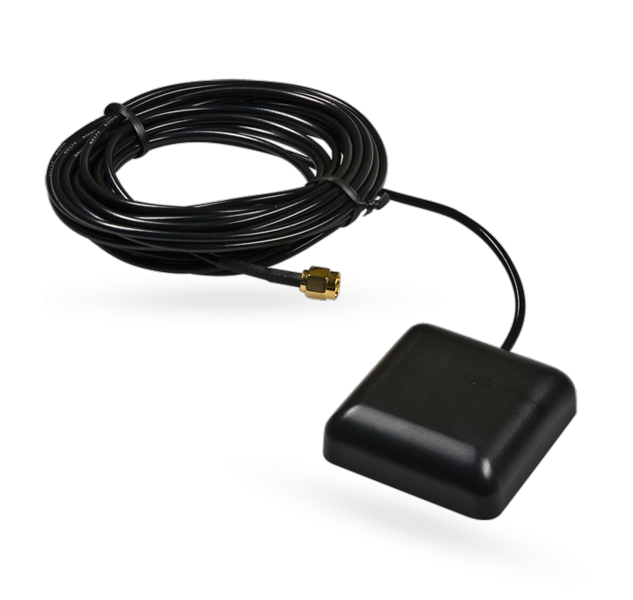
\includegraphics[width=.5\textwidth]{gps-antanna}}
	\caption{آنتن \lr{GPS}}
\end{figure}

\subsection{آنتن \lr{GSM}}
ارتباطات سیستم موقعیت‌بای جهانی وابسته به آنتن می‌باشد. آنتن به سیگنال‌های ارتباطی اجازه می‌دهد، ارسال و دریافت شوند. آنتن مورد استفاده در این پروژه در چهار باند فرکانسی با بهره ۲ دسی‌بل کار می‌کند. (۱۰) در واقع فرکانس کاری آن ۸۹۰، ۹۶۰، ۱۷۱۰، ۱۸۸۰ مگاهرتز می‌باشد. (۱۱)
\\
شکل ۳-۵ برخی از مشخصات آنتن را نشان می‌دهد.(مقاله ۲۰۱۶) و در شکل ۳-۶ این آنتن را مشاهده می‌کنید.
\begin{figure}[!h]
	\centerline{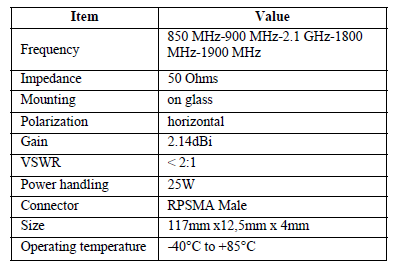
\includegraphics[width=.6\textwidth]{table1}}
	\caption{مشخصات آنتن \lr{GSM}}
\end{figure}
\begin{figure}[!h]
	\centerline{\includegraphics[width=.3\textwidth]{GSM-antenna}}
	\caption{آنتن \lr{GSM}}
\end{figure}

\subsection{اجزاء نرم‌افزاری}
\subsection{نرم‌افزار \lr{Arduino IDE}}
نرم‌افزار مورد استفاده براي برنامه‌ريزي آردوينو، نرم‌افزار  \lr{Arduino IDE} مي‌باشد كه در شکل ۳-۷ نماي كلي از ظاهر اين برنامه را مشاهده مي‌كنيد. با استفاده از زباني شبه \lr{C} ميتوان برنامه مورد نياز را نوشت و بعد از كامپايل، كد هگز توليد شده بر روي آردوينو باز مي‌شود. كتابخانه‌هاي مختلف و متناسب با ماژولٰ‌هاي مختلف وجود دارد كه كدنويسي را راحت‌تر مي‌كند. برای دریافت داده از ماهواره و ارسال آن به تلفن همراه، برنامه با استفاده از ان نرم‌افزار نوشته می‌شود. (\lr{Real Time Google Map and Arduino Based Vehicle	Tracking System})
\begin{figure}[!h]
	\centerline{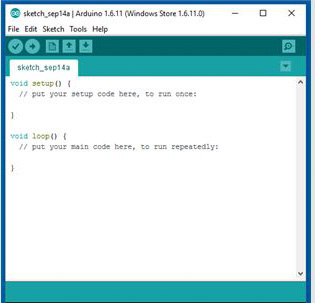
\includegraphics[width=.4\textwidth]{arduino-ide}}
	\caption{نمایی از نرم‌افزار آردوینو}
\end{figure}
\subsection{\lr{google map}}